%!TEX root = Main.tex
\documentclass[Main]{subfiles}

\begin{document}

\section{Software} % (fold)
\label{sec:software}

	In this project, software was a vital part. 
	While the course theory had presented ways of doing 
	In this chapter, the coding environment, structure and behaviour of the codebase will be covered.
	
	\subsection{Environment} % (fold)
	\label{sub:software_environment}

		Here you could write something about c++, Vivado SDK and the compiler that was used.
	
	\subsection{Structure} % (fold)
	\label{sub:software_structure}
	
		The structure of the software will be covered by a class diagram.
		\begin{figure}[H]
			\centering
			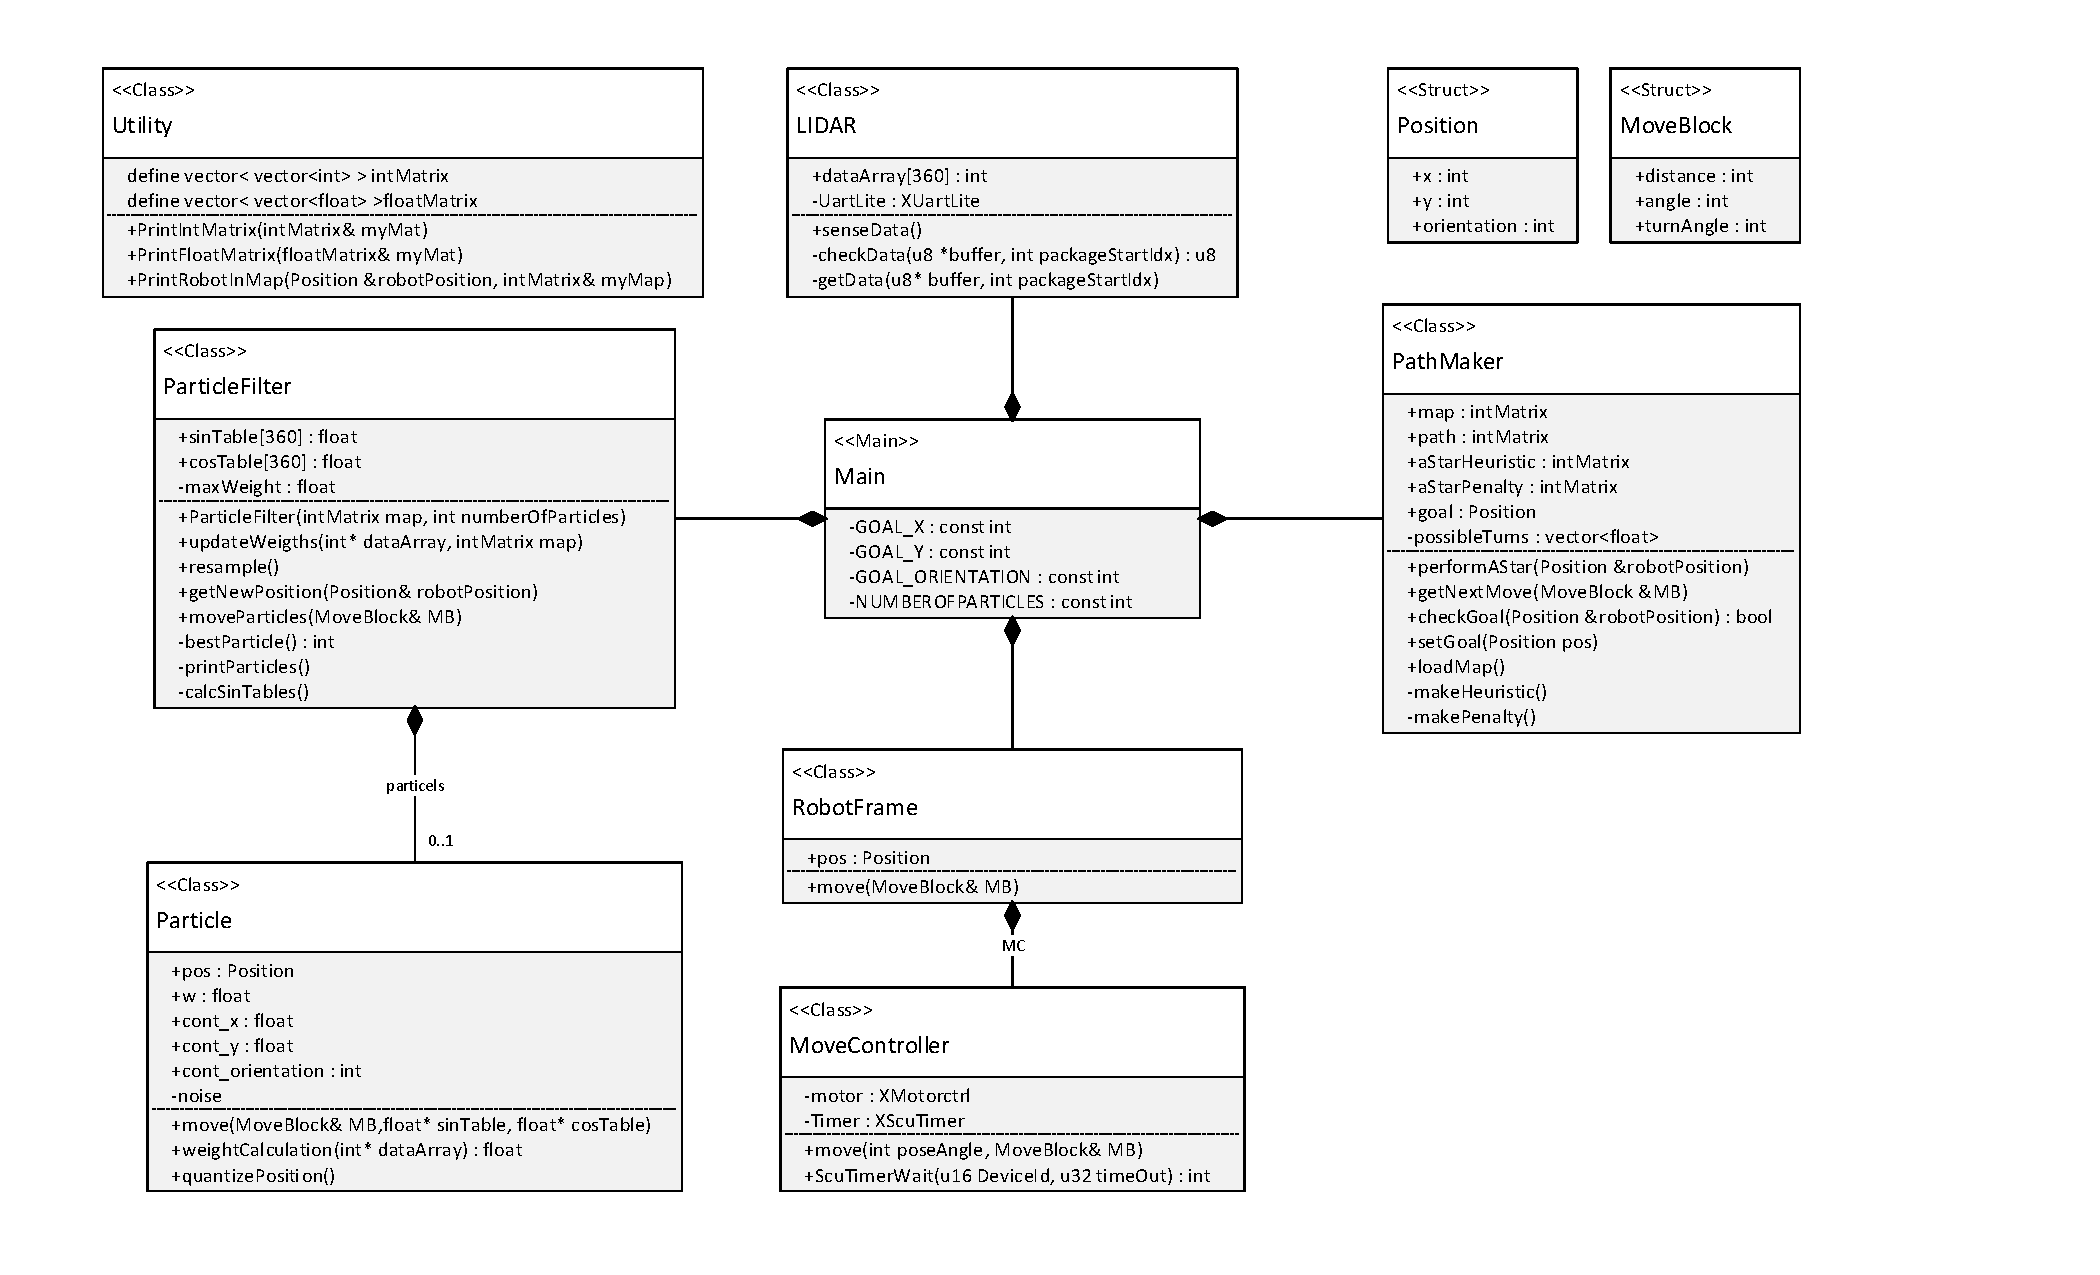
\includegraphics[width=\linewidth]{ClassDiagram}
			\caption{Class Diagram}
			\label{fig:classdiagram}
		\end{figure}

	\subsection{Dataflowyo} % (fold)
	\label{sub:software_dataflow}
		
		The dataflow of the software will be coved by a Internal Block Diagram
		
		\begin{figure}[H]
			\centering
			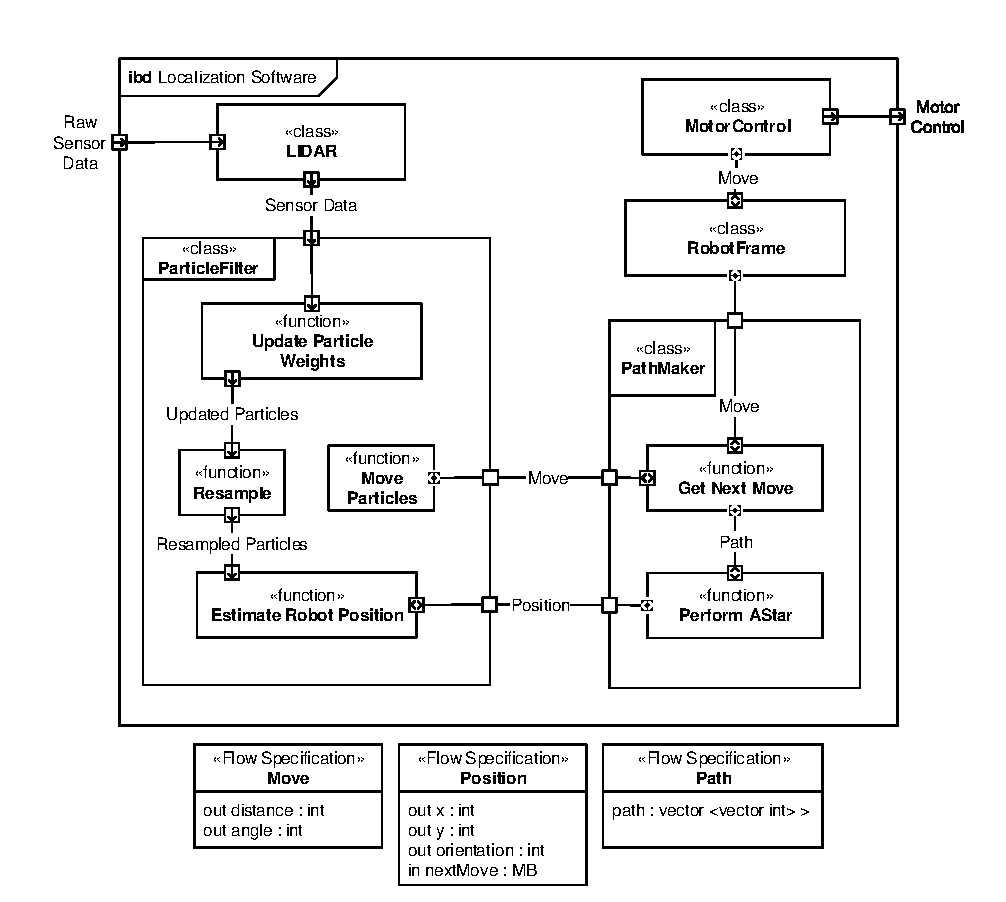
\includegraphics{SoftwareIBD}
			\caption{Software Internal Block Diagram}
			\label{fig:softwareibd}
		\end{figure}

% section software (end)
\end{document}